\section*{Anexos}

% \begin{frame}[noframenumbering]{Anexos}
% \framesubtitle{Comparaci\'on de Herramientas}
% \begin{table}[H]
% \centering
% \footnotesize
% \begin{tabular}{|p{3.5cm}|>{\centering}p{3.5cm}|>{\centering}p{3.5cm}|>{\centering}p{3.5cm}|}
% \hline
%                                & Aplicaciones             &  APIs                            & Librer\'ias/\foreign{Frameworks} \tabularnewline
% \hline
% Conocimiento T\'ecnico         &     Bajo                    & Medio                            & Alto    \tabularnewline \hline
% Productividad                  &     Alto                    & Medio                            & Bajo    \tabularnewline \hline
% Flexibilidad                   &     Bajo                    & Medio                            & Alto    \tabularnewline \hline
% Alternativas  Propietarias      & \begin{itemize} \setlength{\itemsep}{1pt} \setlength{\parskip}{0pt} \setlength{\parsep}{0pt}\item Dragon Natural Speaking \end{itemize}  & \begin{itemize}  \setlength{\itemsep}{1pt} \setlength{\parskip}{0pt} \setlength{\parsep}{0pt} \item Web Speech API \item AT\&T Speech API \item Microsoft Speech API \item iSpeech API \item Dragon Mobile \end{itemize}  &  \tabularnewline \hline
% Alternativas de C\'odigo abierto & \begin{itemize}  \setlength{\itemsep}{1pt} \setlength{\parskip}{0pt} \setlength{\parsep}{0pt} \item Simon \item Palaver \end{itemize}          &           & \begin{itemize} \setlength{\itemsep}{1pt} \setlength{\parskip}{0pt} \setlength{\parsep}{0pt} \item Sphinx 4 \item PocketSphinx \item HTK \item Julius \item Kaldi \end{itemize} \tabularnewline
% \hline
% \end{tabular}
% \caption{Resumen general de las herramientas}
% \label{sec:resumen-herramientas}
% \end{table}
% \end{frame}

\begin{frame}[noframenumbering]{Anexos}
\framesubtitle{Aplicaciones}
\begin{table}[H]
\centering
\footnotesize
\begin{tabular}{|p{2.5cm}|p{2.5cm}|p{2.5cm}|p{2.5cm}|}
\hline
                                      &  Simon                                                       &  Palaver                                       & Dragon Naturally Speaking \\
\hline
Precio                                & Gratuito                                                     & Gratuito                                       & Desde 99\$  \\ \hline
Soporte para m\'ultiples idiomas      & Si                                                           & Si                                             & Si \\ \hline
Facilidad de configuraci\'on          & F\'acil                                    & Reducida                                       & F\'acil \\ \hline
Soporte para dispositivos m\'oviles   & Si                                                           & No                                             & Si, mediante otros productos \\
\hline
\end{tabular}
% \caption{Resumen de los criterios espec\'ificos de las aplicaciones}
\label{sec:resumen-aplicaciones}
\end{table}

\end{frame}

\begin{frame}[noframenumbering]{Anexos}
\framesubtitle{Interfaces de Programaci\'on de Aplicaciones (1/2)}
\begin{table}[H]
\centering
\footnotesize
\begin{tabular}{|p{2.5cm}|p{2.5cm}|p{2.5cm}|p{2.5cm}|}
\hline
                                      &  Web Speech API & AT\&T Speech api & Microsoft Speech API \\
\hline
Empresa o Instituci\'on responsable & \foreign{Speech API Community Group}. Implementado actualmente por \foreign{Google}  &  AT\&T Inc.  & Microsoft\\ \hline
Precio                              & Gratuito, a trav\'es de Google Chrome  & Un mill\'on de llamadas a la API por 99\$ anuales. 0.01\$ por llamada extra  & Gratuito\\ \hline
Soporte para m\'ultiples idiomas    & Si  & 2 idiomas & Si\\ \hline
Soporte Offline                     & No  & No  & Si \\ \hline
Dependencia de Plataforma           & No  & No & Si, solo para \emph{Microsoft Windows} \\
\hline
\end{tabular}
% \caption{Resumen de los criterios espec\'ificos de las APIs. Primera parte.}
\label{sec:resumen-apis}
\end{table}
\end{frame}

\begin{frame}[noframenumbering]{Anexos}
\framesubtitle{Interfaces de Programaci\'on de Aplicaciones (2/2)}
\begin{table}[H]
\centering
\footnotesize
\begin{tabular}{|p{2.5cm}|p{2.5cm}|p{2.5cm}|p{2.5cm}|}
\hline
                                      &  WAMI & iSpeech API & Dragon Mobile \\
\hline
Empresa o Instituci\'on responsable &  \pbox{2.5cm}{Instituto \\ Tecnol\'ogico de Massachusetts} & \foreign{iSpeech}  & \foreign{\pbox{2.5cm}{Nuance \\ Communications}} \\ \hline
Precio &  Gratuito  & Gratuito para aplicaciones no comerciales. De 0.02\$ a 0.0001\$ para otros usos & Gratuito para aplicaciones no comerciales. De 0.08\$ a 0.006\$ para otros usos. \\ \hline
Soporte para m\'ultiples idiomas  & No, aunque depende del reconocedor utilizado & Si & Si \\ \hline
Soporte Offline & No & No & No\\ \hline
Dependencia de Plataforma & No & No & No\\
\hline
\end{tabular}
% \caption{Resumen de los criterios espec\'ificos de las APIs. Segunda parte.}
\label{sec:resumen-apis-2}
\end{table}
\end{frame}

\begin{frame}[noframenumbering]{Anexos}
\framesubtitle{Librer{\'\i}as (1/2)}
\begin{table}[H]
\centering
\footnotesize
\begin{tabular}{|p{2.5cm}|p{2.5cm}|p{2.5cm}|p{2.5cm}|}
\hline
                                  &  Sphinx 4 & PocketSphinx & HTK \\
\hline
Empresa o Instituci\'on Responsable & \pbox{2.5cm}{Universidad \\ \foreign{Carnegie Mellon}} & \pbox{2.5cm}{Universidad \\ \foreign{Carnegie Mellon}} & Universidad de Cambridge \\ \hline
Precio & Gratuito & Gratuito & Gratuito \\ \hline
Licencia & BSD, con un componente privativo & BSD simplificada & C\'odigo fuente modificable, se prohibe redistribuci\'on.\\ \hline
Soporte para m\'ultiples idiomas & Si & Si & No\\ \hline
Dependencia de Plataforma & No & No & No \\ \hline
Modelos de Lenguaje Aceptados & JGSF, bigramas y trigamas &  JGSF, bigramas y trigamas &  JGSF, bigramas y trigamas \\ \hline
Modelos Ac\'usticos Aceptados & Modelo propio & Modelo propio &  Modelo propio \\ \hline
Uso de Memoria & No se recomienda para sistemas de poca memoria & Reducido en comparaci\'on a Sphinx 4 & Dependiente de la aplicaci\'on \\
\hline
\end{tabular}
% \caption[Resumen de los criterios espec\'ificos de las Librer\'ias/\foreign{Frameworks}.\protect\newline Primera parte.]
% {Resumen de los criterios espec\'ificos de las Librer\'ias/\foreign{Frameworks}. Primera parte.}
\label{sec:resumen-libs}
\end{table}


\end{frame}

\begin{frame}[noframenumbering]{Anexos}
\framesubtitle{Librer{\'\i}as (2/2)}
\begin{table}[H] 
\centering
\footnotesize
\begin{tabular}{|p{2.5cm}|p{2.5cm}|p{2.5cm}|}
\hline
                                  &  Julius & Kaldi \\
\hline
Empresa o Instituci\'on Responsable &  \foreign{Interactive Speech Technology Consortium} & Agencia Tecnol\'ogica de Rep\'ublica Checa \\ \hline
Precio & Gratuito & Gratuito \\ \hline
Licencia & BSD & Apache 2.0 \\ \hline
Soporte para m\'ultiples idiomas & No &  No \\ \hline
Dependencia de Plataforma & No & No \\ \hline
Modelos de Lenguaje Aceptados & Basados en gram\'aticas y modelos en formato ARPA & Modelos en formato FST \\ \hline
Modelos Ac\'usticos Aceptados & Modelo propio & Modelo propio \\ \hline
Uso de Memoria & Bajo & \\
\hline
\end{tabular}
% \caption[Resumen de los criterios espec\'ificos de las librer\'ias/\foreign{framework}s.\protect\newline Segunda parte.]{Resumen de los criterios espec\'ificos de las librer\'ias/\foreign{framework}s. Segunda parte.}
\label{sec:resumen-libs-2}
\end{table}
\end{frame}

\begin{frame}[noframenumbering]{Anexos}
\framesubtitle{Ecuaci\'on Fundamental del Reconocimiento del Habla}
\begin{align*}
\hat{W} = \argmax_{W \in L} P(W|O)
\end{align*}

Usando la Regla de Bayes puede reescribirse como:

\begin{align*}
\hat{W} = \argmax_{W \in L} \frac{P(O|W)P(W)}{P(O)}
\end{align*}

Se busca la oraci\'on con mayor probabilidad dada una entrada ac\'ustica,
la misma para todas las oraciones evaluadas.
En otras palabras, el t\'ermino $P(O)$ es independiente de $W$. Por tanto:

\begin{align*}
\hat{W} = \argmax_{W \in L} P(O|W)P(W)
\end{align*}

\end{frame}

\begin{frame}[noframenumbering]{Anexos}
\framesubtitle{Escala de Mel}
\begin{figure}[H]
\centering
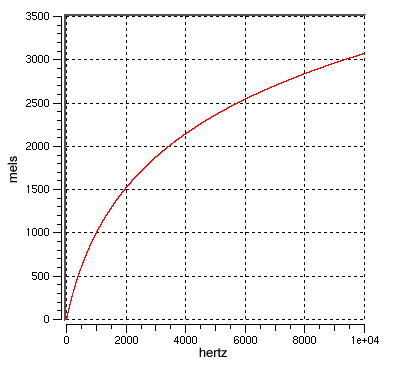
\includegraphics[width=0.7\linewidth]{./graphics/mel_hz.png}
\end{figure} 
\end{frame}

\begin{frame}[noframenumbering]{Anexos}
\framesubtitle{Algoritmo de Viterbi (1/4)}
El algoritmo utiliza una matriz de probabilidades $viterbi$, donde cada celda $viterbi[i,t]$ 
contiene la probabilidad del mejor camino teniendo en cuenta las $t$ primeras observaciones y 
terminando en el estado $i$ del modelo.

\begin{align*}
    viterbi[i,t] = \displaystyle \underset{q_1,q_2,\ldots,q_{t - 1}}{max} P(q1,q2,\ldots,q_{t - 1},
        q_t = i,o_1,o_2,\ldots,o_t \mid \lambda)    
\end{align*} 

Para calcular los valores de $viterbi[i,t]$, el algoritmo de Viterbi asume la invariante de la 
programaci\'on din\'amica. Esto es, se asume que si el mejor camino para una secuencia de observaciones 
pasa por un estado $q_i$, entonces este camino incluye el mejor camino hasta $q_i$ inclusive. 


\begin{align*}
    viterbi[i,t] = \displaystyle \underset{i}{max} (viterbi[i,t-1]a_{i,j})b_j(o_t)
\end{align*}

\end{frame}

\begin{frame}[noframenumbering]{Anexos}
\framesubtitle{Algoritmo de Viterbi (2/4)}

\begin{algorithm}[H]
\footnotesize
\caption{Algoritmo de Viterbi} \label{viterbi}
\begin{algorithmic}[1]
\REQUIRE $observaciones$ de longitud $T$, $grafo\mbox{-}estados$.
\ENSURE $estados$, el mejor camino.
\STATE $num\mbox{-}estados \leftarrow$ CANTIDAD-DE-ESTADOS($grafo\mbox{-}estados$) 
\STATE Crear una matriz de probabilidades $viterbi[num\mbox{-}estados, T]$
\FOR{cada estado $s$ desde $0$ hasta $num\mbox{-}estados$}
    \STATE $viterbi[s,0] = \pi_s$
\ENDFOR
\FOR{cada paso $t$ desde $0$ hasta $T - 1$}
    \FOR{cada estado $s$ desde $0$ hasta $num\mbox{-}estados$}
        \FOR{cada transici\'on $s'$ desde s especificada por el $grafo\mbox{-}estados$}
        \STATE $nuevo\mbox{-}puntaje \leftarrow viterbi[s,t] * a[s,s'] * b_{s'}[o_t]$
        \IF{$viterbi[s',t+1] = 0 \parallel nuevo\mbox{-}puntaje > viterbi[s',t+1]$}
            \STATE $viterbi[s',t+1] \leftarrow nuevo\mbox{-}puntaje$
            \STATE $puntero\mbox{-}retroceso[s',t+1] \leftarrow s$
        \ENDIF  
        \ENDFOR
    \ENDFOR
\ENDFOR
\STATE $estados \leftarrow$ retroceso desde la celda con mayor valor en la \'ultima columna de $viterbi[]$
\COMMENT{Usando $puntero-retroceso$}.
\RETURN $estados$
\end{algorithmic}
\end{algorithm}
\end{frame}

\begin{frame}[noframenumbering]{Anexos}
\framesubtitle{Algoritmo de Viterbi (3/4)}
\begin{figure}[H]
\centering
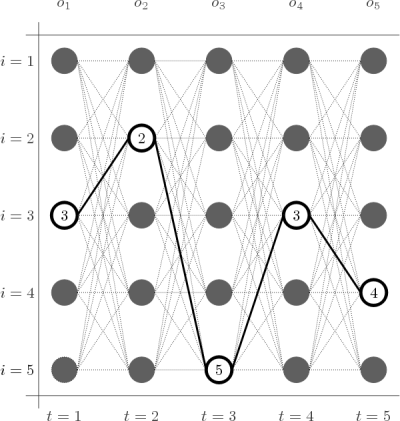
\includegraphics[width=0.6\linewidth]{./graphics/hmm-viterbi2.png}
\end{figure}
\end{frame}

\begin{frame}[noframenumbering]{Anexos}
\framesubtitle{Algoritmo de Viterbi (4/4)}
\begin{figure}[H]
\centering
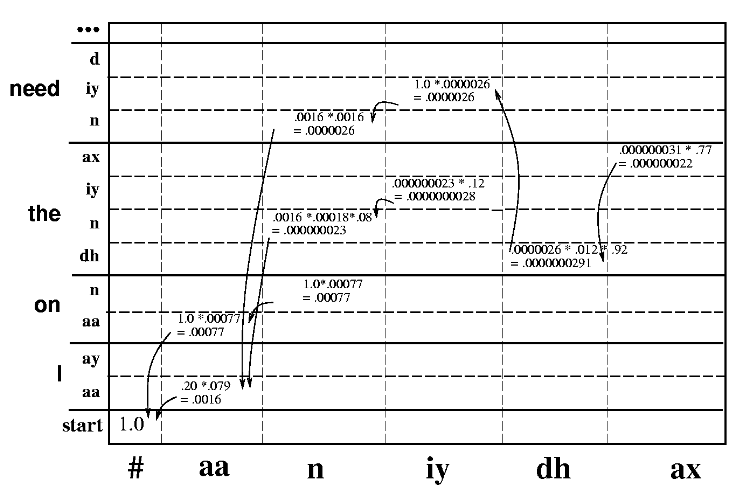
\includegraphics[width=1\linewidth]{./graphics/viterbi3.png}
\end{figure}
\end{frame}

\begin{frame}[noframenumbering]{Anexos}
\framesubtitle{Entrenamiento (1/4)}
%\subsection*{Modelo de Lenguaje}

El modelo se entrena contando las ocurrencias de cada n-grama en el corpus de texto, para luego
normalizar el conteo dividiendo sobre la cantidad total de n-gramas en el corpus.
A continuaci\'on se utilizan normalmente m\'etodos de reestimaci\'on, de modo a mejorar las estimaciones 
de n-gramas con un conteo muy bajo, o incluso igual a cero. Este proceso se conoce como suavizamiento
del modelo.

Finalmente, el conteo normalizado y suavizado de cada n-grama en el corpus del texto constituye su
probabilidad \cite{CollinsLanguage}.

\end{frame}

\begin{frame}[noframenumbering]{Anexos}
\framesubtitle{Entrenamiento (2/4)}

%\subsection*{HMM: Estructura del grafo de estados}
El conjunto de estados de cada HMM, $S$, y las transiciones entre estos estados se definen en base
al diccionario fon\'etico. A modo de ejemplo, \mbox{CMUdict \cite{CMUdict}} es un diccionario fon\'etico
que contiene correspondencias entre palabras y las secuencias de fonemas que las componen para m\'as de
125.000 palabras del idioma ingl\'es.

\begin{figure}[H]
\centering
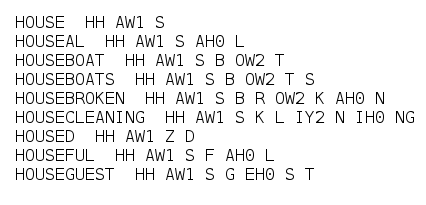
\includegraphics[width=0.8\linewidth]{./graphics/diccionario.png}
\end{figure}
\end{frame}

\begin{frame}[noframenumbering]{Anexos}
\framesubtitle{Entrenamiento (3/4)}
Para cada HMM es necesario estimar los siguientes par\'ametros:
    \begin{itemize}
        \item Las probabilidades de estado inicial: $\pi_i$
        \item Las probabilidades de transici\'on: $a_{ij}$
        \item Las probabilidades de observaci\'on: $b_j(o_t)$ 
    \end{itemize}

Para esto se cuenta con \cite{Jurafsky}:
    \begin{itemize}
        \item  Un corpus de voz, compuesto por una colecci\'on de grabaciones de voz junto
        con sus transcripciones de texto.
        \item Un corpus de voz de menor tama\~no etiquetado fon\'eticamente. 
        Esto es, donde fragmentos de la se\~nal est\'an asociados a su fonema correspondiente.
    \end{itemize}

\end{frame}

\begin{frame}[noframenumbering]{Anexos}
\framesubtitle{Entrenamiento (4/4)}

Para las probabilidades de estado inicial, se asume que cualquier estado es igualmente probable 
como estado inicial. De manera similar, para las probabilidades de transici\'on se asume que, para cada estado, cualquier transici\'on a otro estado es igualmente probable.

Las probabilidades de observaci\'on se estiman inicialmente mediante el peque\~no corpus 
de voz etiquetado fon\'eticamente.

La siguiente etapa var{\'\i}a de acuerdo al m\'etodo escogido para la definici\'on de las probabilidades
de observaci\'on, $b_j$. Si se utilizan funciones Gaussianas, el cual constituye el caso m\'as
frecuente, las estimaciones iniciales se mejoran mediante el algoritmo de Baum--Welch.

El algoritmo de Baum--Welch calcula dos probabilidades adicionales en base a las estimaciones
iniciales de $a_{ij}$ y $b_j(o_t)$, denominadas probabilidad de avance y probabilidad de retroceso. 
Utilizando estas probabilidades, se mejoran las estimaciones $a_{ij}$ y $b_j(o_t)$ mediante
un proceso iterativo que se repite hasta que los valores converjan \cite{Rabiner89atutorial}.
\end{frame}

\begin{frame}[noframenumbering]{Anexos}
\framesubtitle{Algoritmo de Baum--Welch}
\begin{figure}[H]
\centering
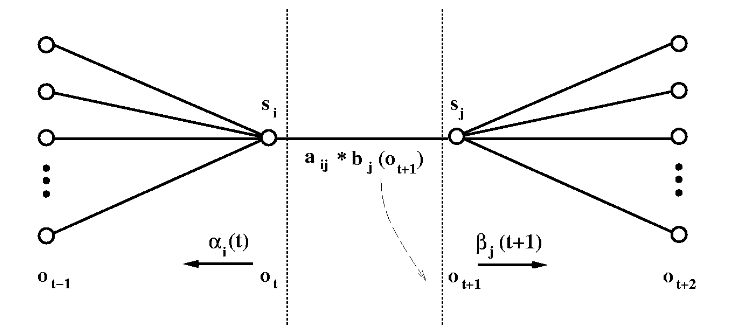
\includegraphics[width=1\linewidth]{./graphics/forward-backward.png}
\end{figure}
\end{frame}

\begin{frame}[noframenumbering]{Anexos}
\framesubtitle{Dynamic Time Warping}
\begin{figure}[H]
\centering
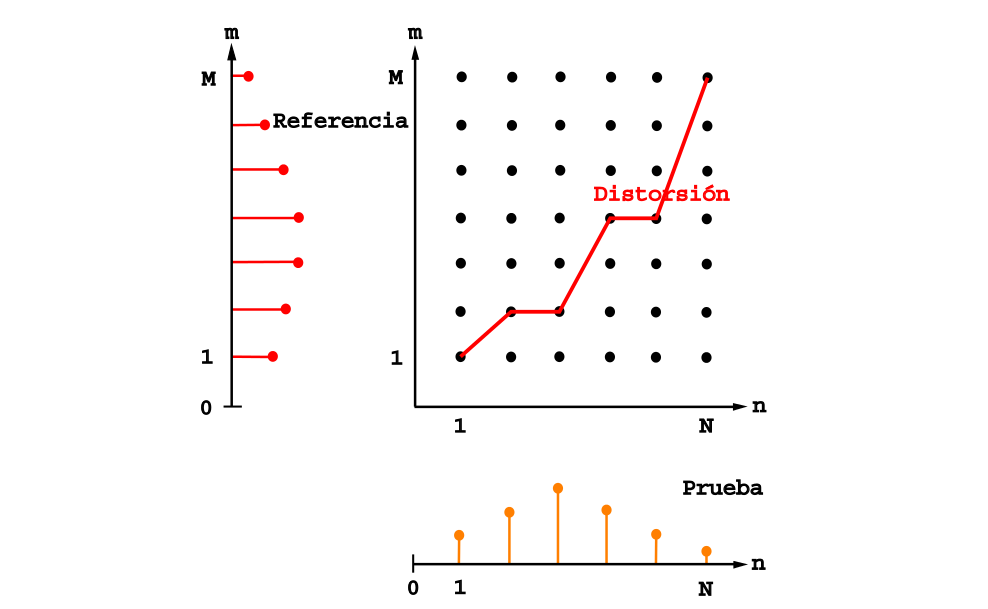
\includegraphics[width=1\linewidth]{./graphics/dtw-anexos.png}
\end{figure}
\end{frame}

\begin{frame}[noframenumbering]{Anexos}
\framesubtitle{Tamaño de Muestra (1/2)}
We do have some useful advice from the research community that a study utilizing 8-25 participants per group is a sensible range to consider and that 10-12 participants is probably a good baseline range.
(\textit{How To Specify the Participant Group Size for Usability Studies: A Practitioner’s Guide}, Macefield, 2009)
\end{frame}


\begin{frame}[noframenumbering]{Anexos}
\framesubtitle{Tamaño de Muestra (2/2)}
\begin{figure}[H]
\centering
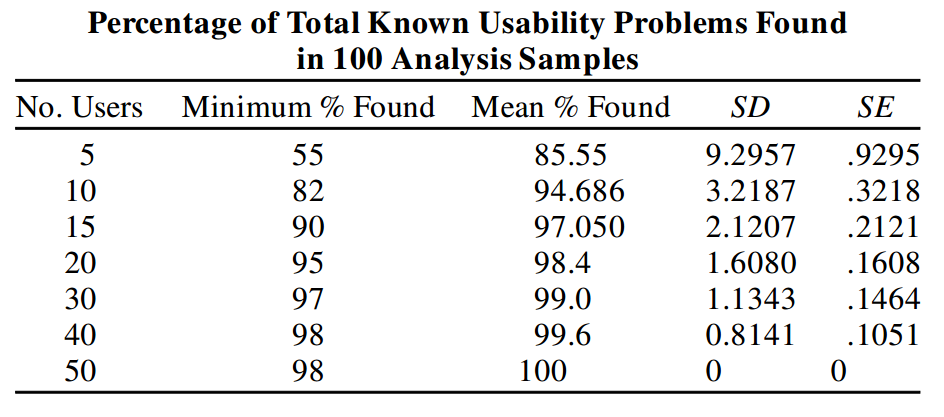
\includegraphics[width=1\linewidth]{./graphics/groupsize.png}
\caption{\textit{Beyond the five-user assumption: Benefits of
increased sample sizes in usability testing}, Faulkner, 2003}
\end{figure}
\end{frame}

\begin{frame}[noframenumbering]{Anexos}
\framesubtitle{Coeficientes de Correlaci\'on de Pearson}
El coeficiente de Pearson es una medida del grado de correlaci\'on lineal o dependencia entre dos 
variables $X$ e $Y$. El valor del coeficiente se encuentra entre -1 y 1 inclusive. 
El valor -1 indica que las variables est\'an correlacionadas negativamente 
(cuando $X$ crece, $Y$ decrece y viceversa), 0 indica que no existe correlaci\'on y 1 que existe una 
correlaci\'on positiva (cuando $X$ crece, $Y$ crece).
\end{frame}

\begin{frame}[noframenumbering]{Anexos}
\framesubtitle{Satisfacci\'on del Usuario (1/2)}
La opini\'on del usuario se mide a trav\'es de los resultados de la encuesta que se realiza como parte de
la prueba de usabilidad, posterior a la finalizaci\'on de las tareas. Las respuestas se
registran utilizando una escala de Likert con valores del 1 al 7.
\end{frame}

\begin{frame}[noframenumbering]{Anexos}
\framesubtitle{Satisfacci\'on del Usuario (2/2)}
Posteriormente, de modo a eliminar el potencial efecto de los estilos de respuesta
de los usuarios, se utiliza el m\'etodo de estandarizaci\'on 
por rango para reescalar los resultados de la encuesta.

Siendo:
\begin{itemize}
	\item $min_i$ la respuesta de menor valor del usuario $i$.
	\item $max_i$ la respuesta de mayor valor del usuario $i$.
\end{itemize}

Para cada respuesta $s$ del usuario $i$, el valor ajustado $s_a$ se define como:

\begin{equation*}
s_a=\frac{s-min_i}{max_i-min_i}
\end{equation*}


De esta manera, todas las respuestas pasan a estar en el rango entre 0 y 1.  
\end{frame}